\documentclass{article}
% packages
\usepackage {lmodern}
\usepackage [T1]{fontenc}
\usepackage {amsmath}
\usepackage {amssymb}
\usepackage {amsfonts}
\usepackage {graphicx}
\usepackage {fullpage}
\usepackage {gensymb}
\usepackage {caption}
%\usepackage{nopageno}
\usepackage {cite}
\usepackage {setspace}
\usepackage [version=4]{mhchem}

% graphics path
\graphicspath {{images/}}

%begin document
\begin {document}
\title {Preparation of a NaOH Standard Solution and \\ Determination of Aspirin
Content} 
\author {Justin Chao - jc55395 \\ \\ CH 456}
\maketitle

\vspace {50mm}
%\section* {Abstract} %optional

\newpage
\doublespacing
\section {Introduction}
This experiment aims to determine the acetyl salicylic acid content in an analgesic tablet. 
A standardization of an NaOH solution by direct titration against KHP is performed as well.

\subsection{Using a Burette}
In a titration, increments of a reagent solution, called the titrant, are added to the analyte until
the reaction has proceeded to completion. The titrant is usually added from a burette, which allows
for an accurate measurement of the volume of titrant added.\cite{Harris}
Figure 1 provides an illustration of a burette.
\begin{center}
        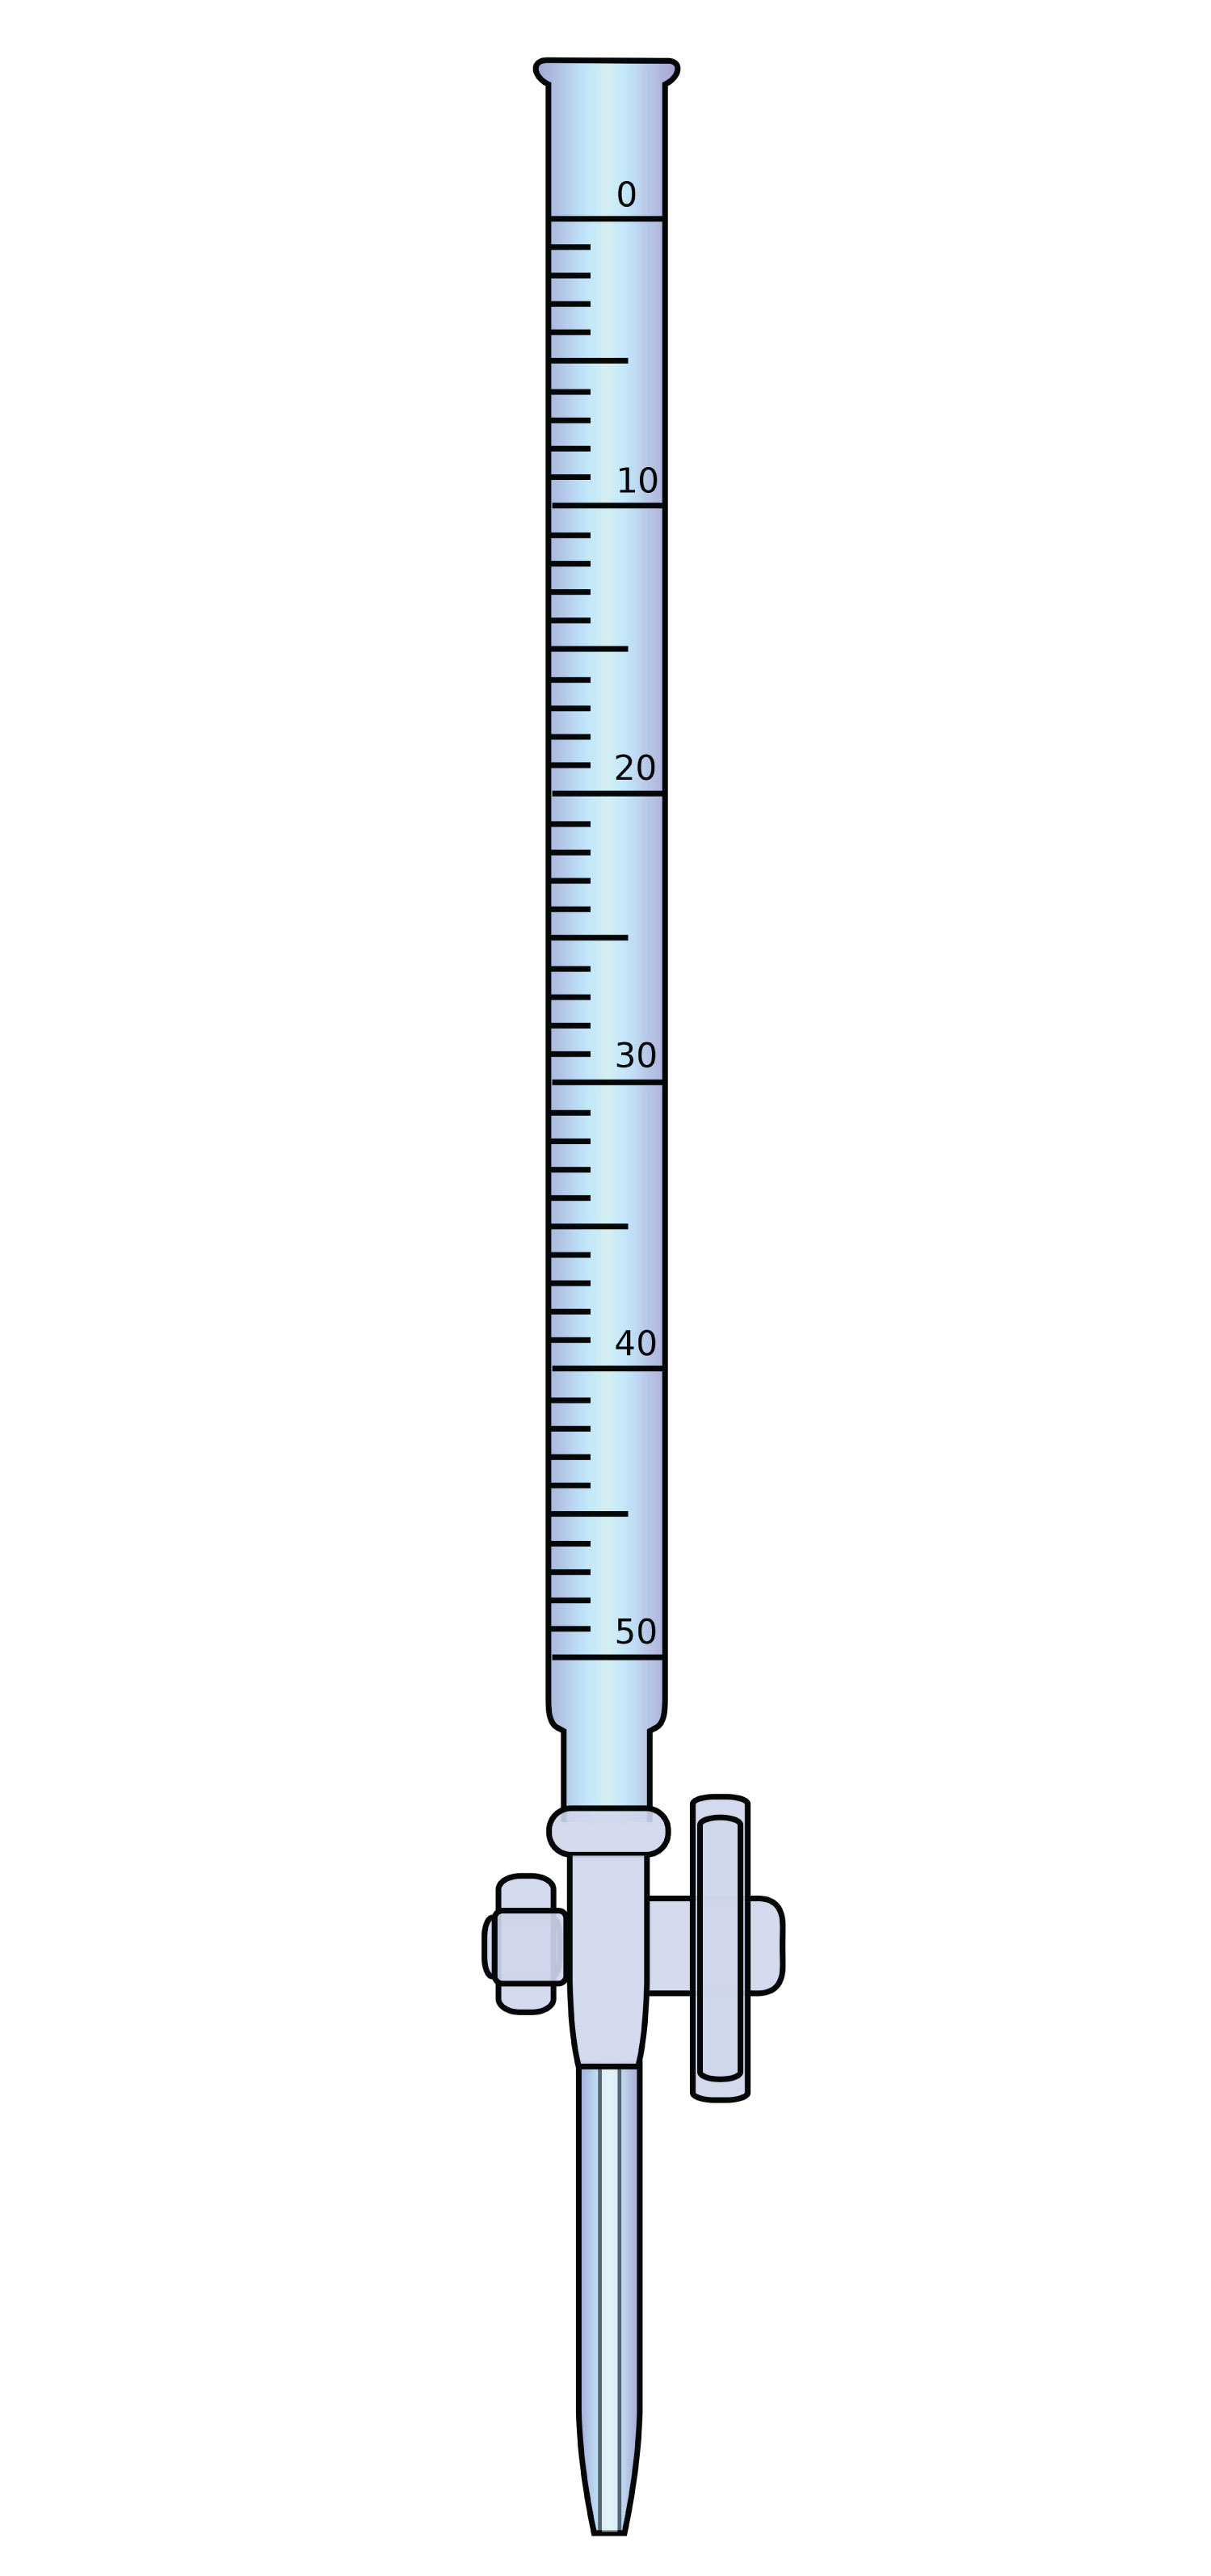
\includegraphics[scale = 0.05]{buret}
        \captionof{figure}{Illustration of burette. \cite{buret}}
\end{center}

The burette is usually glass so that the liquid inside can be observed easily.
The numbers on a burette are labled "backwards", with "0" at the top and
increasing as they proceed down the side. In this manner, it is easy to measure
the amount of titrant used by subtracting the final volume remaining in the
burette from the initial volume. There is a valve at the bottom of the burette
that allows the titrant to be released ranging from a steady flow to a single
drop. Controlling the level of flow is essential in ensuring that an accurate
measurement of titrant needed for the reaction to proceed to completion is
taken.

\subsection{Standardization of NaOH by Direct Titration}
In determining when the reaction is complete, an indicator (or some reagent) is used to monitor the
reaction progress. In this experiment, phenolphthalein is used as a pH indicator to monitor the
progress of the acid-base reaction. Phenolphthalein, hereafter abbreviated as phph, remains
colorless in acidic solutions, but it turns pink in basic solutions. Figure 2 illustrates the
chemical structure of phph. Figure 3 illustrates the changes that different pH indicators can go
through under different pH conditions.
\begin{center}
        
\includegraphics[scale=0.6]{phph}
        \captionof{figure}{Structure of Phenolphthalein. \cite{phph}}
        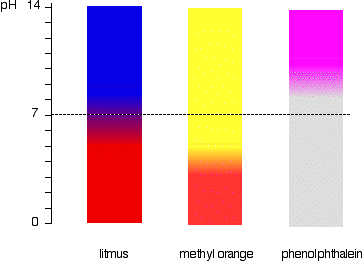
\includegraphics[scale=0.5]{phph_color}
        \captionof{figure}{Color changes of litmus, methyl orange, and phenolphthalein indicators.
        \cite{phph_color}}
\end{center}

The equivalence point is the point at which the volume of titrant that is added is exactly
equivalent to the amount that is necessary to balance the analyte. In the case of an acid-base
reaction, the equivalence point is reached when the pH has been exactly neutralized.
Due to the accuracy that is required in determining the equivalence point, there is an amount of
uncertainty that is involved. Especially when titrating with a visual indicator such as
phenolphthalein, titrations are performed until a visible color change is noted, at which point the
reaction has proceeded past the equivalence point already. 
The end point is the point at which there is an observed change in solution. In this experiment, the
end point is reached once there is a visible color change from the phph indicator. \cite{aspirin_rxn}

In this experiment, a solution of NaOH is standardized by direct titration against KHP.
KHP is a good option as a primary standard due to its availability in high purity. It is also
non-hydroscopic and not easily oxidized by air. KHP is soluble in water, and proceeds
stoichiometricly and instantaneously in reactions.
Figure 4 illustrates the reaction between KHP and NaOH.
\begin{center}
        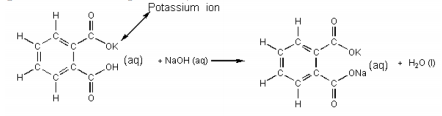
\includegraphics[scale=1]{KHP_rxn}
        \captionof{figure}{Neutralization reaction of potassium hydrogen phthalate with sodium
        hydroxide, forming sodium potassium phthalate and water. \cite{aspirin_rxn}}
\end{center}

\subsection{Determination of Aspirin Content by Back Titration}

In a  back titration, excess reagent is added to the analyte to force the reaction towards
completion by le Chatelier's principle of equilibrium. The excess amount of this added reagent is
then determined by a "back titration". In this experiment, an excess amount of NaOH is added to the
sample of aspirin, and a back titration is conducted using HCl. The excess amount of NaOH that
remains unreacted can then be calculated from the amount of HCl used in the back titration.
\cite{lab_man}

This method of titration is useful for reactions that can proceed through multiple
pathways. Due to the level of uncertainty involved in determining if a particular reaction has
proceeded to completeness, it can be difficult to deterine the end point by direct
titration.\cite{lab_man} In this experiment, the reaction of acetyl salicylic acid with NaOH can
proceed via a fast acid-base reaction and a slow hydrolysis reaction. Figure 5 illustrates these
two different reactions.

\begin{center}
        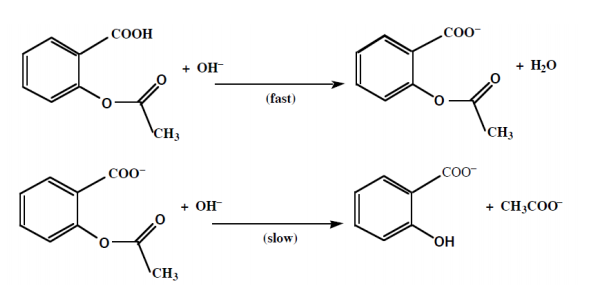
\includegraphics[scale=0.5]{aspirin_rxn}
        \captionof{figure}{Reaction pathways of aspirin with a base. \cite{aspirin_rxn}}
\end{center}

%\section {Experimental} %optional
\newpage

\section {Results and Discussion}

Tables 1 and 2 show the calculated results of the concentration of NaOH and Aspirin content for each
trial.
\begin{center}
        \begin{tabular}{ |c|c|c|c| }
                \hline
                & Trial 1 & Trial 2 & Trial 3 \\
                \hline
                [NaOH] & 0.091 M & 0.095 M & 0.093 M \\
                \hline
        \end{tabular}
        \captionof{table}{Calculated concentration of NaOH per trial.}
        \vspace{1cm}

        \begin{tabular}{ |c|c|c|c| }
                \hline
                & Trial 1 & Trial 2 & Trial 3 \\
                \hline
                Mass of Aspirin & 0.34 g & 0.34 g & 0.36 g \\ 
                \hline
        \end{tabular}
        \captionof{table}{Calculated mass of Aspirin per trial.}
\end{center}

Tables 3, 4, and 5 show the results of the calculated concentration of NaOH and Aspirin content,
compiled from three trials.
\begin{center}

        \begin{tabular}{ |c|c|c|c| }
                \hline
                [NaOH] & Standard Deviation & RSD & 90\% Confidence Interval \\
                \hline
                0.093 M & 0.002 & 0.093 M $\pm$ 2.2\% & 0.093 M $\pm$ 0.003 \\
                \hline
        \end{tabular}
        \captionof{table}{Average concentration of NaOH.}
        \vspace{1cm}
        
        \begin{tabular}{ |c|c|c|c| }
                \hline
                Percent mass of Aspirin & Standard Deviation & RSD & 90\%
                Confidence Interval \\
                \hline
                88\% & 2.6 & 88\% $\pm$ 3\% & 88\% $\pm$ 2.5 \\
                \hline
        \end{tabular}
        \captionof{table}{Average percent mass of Aspirin per tablet.}
        \vspace{1cm}

        \begin{tabular}{ |c|c|c|c| }
                \hline 
                Mass of Aspirin & Standard Deviation & RSD & 90\% Confidence Interval \\
                \hline
                350 mg & 0.01 & 350 mg $\pm$ 3\% & 350 mg $\pm$ 20 \\
                \hline
        \end{tabular}
        \captionof{table}{Average mass of Aspirin per tablet.}
\end{center}

Please refer the the Appendix for detailed calculations in determining results and statistics.

The calculated results for each of the trials show an acceptable level of
precision in the end results.  The concentration of NaOH used in this experiment
was reported to be approx. 0.1 M. The standardized concentration of NaOH was
determined to be 0.093 M with a 90\% confidence interval of $\pm$ 0.003. The
unknown solution of NaOH used was Unknown F.  This is slightly under the
reported value of 0.1 M, and this deviation in accuracy can be attributed to
different levels of precision in the values of molar mass used in calculating
the concentration of NaOH. This may also be a result of systematic error in the
precisions used when weighing the mass of KHP.

The sample of Aspirin used in this experiment was from a CVS brand, reported to contain 325 mg of
aspirin per tablet. The experimentally determined amount of Aspirin was 350 mg with a 90\%
confidence interval of $\pm$ 20.
This is slightly under the reported mass of 325 mg, and the deviation can also be attributed
systematic error in the precisions used when weighing the Aspirin tablets.

Improvement that could be made to increase the accuracy of the experiment may include the inclusion
of more trials. The pre-heating of lab glassware to remove any water particles may also increase
the accuracy of the experiment.

\section {Conclusion}

The concentration of NaOH was determined to be 0.093 M $\pm$ 0.003 with a confidence interval of
90\% by direct titration against KHP. The mass of Aspirin per tablet was determined to be 350 mg
$\pm$ 20 with a confidence interval of 90\%, using back titration. The results of all three trials
conducted show an acceptable level of precision and repoducibility. The average results of all three
trials are within a reasonable margin of error. The small degree of error in accuracy when comparing
the mass of Aspirin calculated to the reported mass of 325 mg can be attributed to systematic errors
in levels of precision used.


\newpage
\bibliographystyle{unsrt}
\bibliography{aspirin.bib}
\newpage

\section {Appendix}

\begin{enumerate}
        \item Lab notebook pages with calculations.
\end{enumerate}

\end {document}
